\chapter{Cathode Rays}\label{ch:thomson}

\chapterprecis{J.\ J.\ Thomson}

\makeoddhead{myheadings}{\emph{Thomson}}{}{\thepage}
\makeevenhead{myheadings}{\thepage}{}{\emph{Cathode Rays}}

\renewcommand{\theequation}{\arabic{equation}}

\section*{Remarks}

\begin{wrapfigure}[8]{r}{0.33\textwidth}
  \begin{center}
    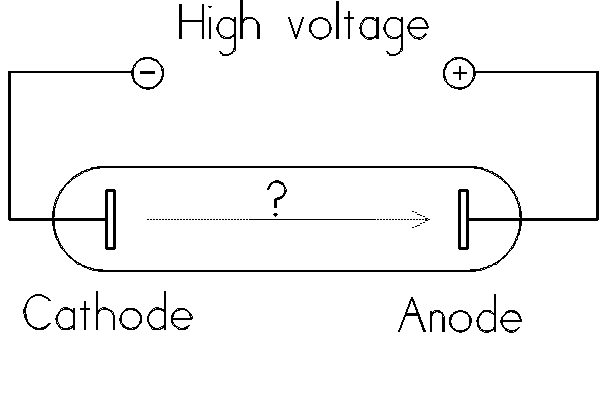
\includegraphics[width=2in,height=1.26042in]{images/02_thomson/image001.png}
  \end{center}
\end{wrapfigure}

\indent

We pursue
further the investigation of ``charge,'' particularly its relation to
matter. An avenue for investigation of this question was opened by the
discovery of the so-called ``cathode rays.'' If a glass tube into which
two electrodes had been sealed was evacuated, and if a high potential
difference was placed across the two electrodes, a mysterious emanation
issued from the cathode (negative electrode), evidenced, among other
manifestations, by its ability to cause phosphors and even certain types
of glass to \emph{glow}. These rays, like the ionic motions in
electrolysis, served to complete the circuit and thus in a sense to
``separate the current from the wire'' and make it available for
independent study. J.\ J.\ Thomson, making the initial hypothesis that the
rays consisted of a flow of electrified particles, showed that they did
indeed exhibit properties of both mass and charge, related in a definite
manner.
\begin{wrapfigure}[8]{l}{0.33\textwidth}
  \begin{center}
    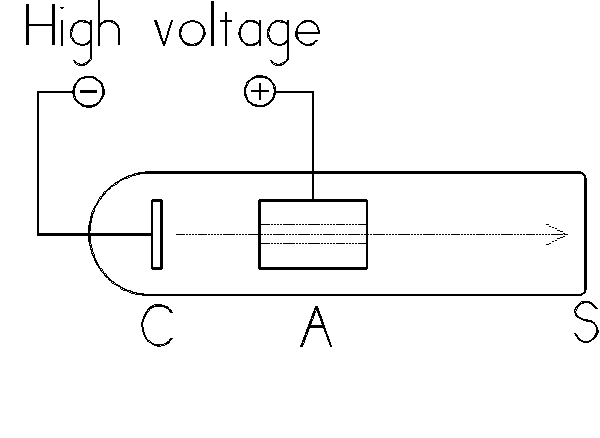
\includegraphics[width=1.9in,height=1.26042in]{images/02_thomson/image003.png}
  \end{center}
\end{wrapfigure}

Thomson's
1897 paper on cathode rays is reproduced in part below. He assumes the
reader to be familiar with the cathode ray phenomenon. We have sketched
two forms of the cathode-ray apparatus here. First depicted is the
simplest version: C is the cathode and A the anode of an evacuated tube.
The anode contains a small slit; and that a ray of some sort passes
through the slit is shown by a bright spot on the zinc sulfide screen S.
The spot (and hence the ``ray'') can be deflected by bringing a magnet
near the tube in the region between A and S.


\begin{wrapfigure}[8]{r}{0.33\textwidth}
  \begin{center}
    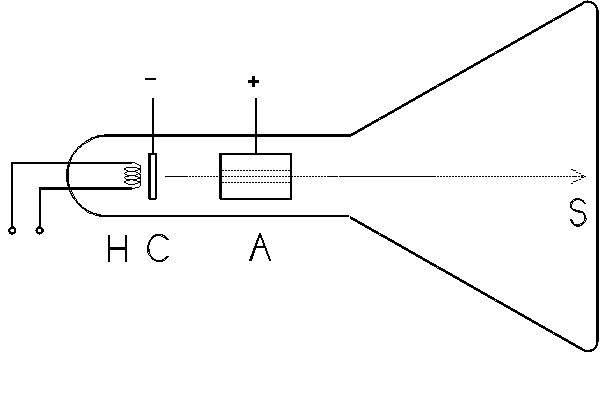
\includegraphics[width=2in,height=1.25in]{images/02_thomson/image005.png} 
  \end{center}
\end{wrapfigure}
The next sketch shows a modern form of cathode-ray tube, much like an
oscilloscope or television picture tube. Here H is an
electrically-heated wire mounted close to cathode C, for it is found
that production of rays is greatly increased if the cathode is heated.
One cylindrical anode A is drawn in the figure, but in practice
additional anodes are sometimes used to bring the beam to a sharp focus
on screen S. The beam may be deflected magnetically or, as Thomson
shows, electrostatically. It becomes then a delicate and versatile
pencil capable of drawing patterns on the screen which faithfully
reflect conditions in the circuits governing the electric or magnetic
deflection.


\section*{Cathode Rays\footnote{{[}\emph{Philosophical Magazine}, \textbf{44}
 (1897), 293--311.{]}}\\ {\large J.\ J.\ Thomson}}


The experiments discussed in this paper were undertaken in the hope of
gaining some information as to the nature of the Cathode Rays. The most
diverse opinions are held as to these rays; according to the almost
unanimous opinion of German physicists they are due to some process in
the æther to which---inasmuch as in a uniform magnetic field their
course is circular and not linear---no phenomenon hitherto observed is
analogous: another view of these rays is that, so far from being wholly
ætherial, they are in fact wholly material, and that they mark the paths
of particles of matter charged with negative electricity. It would seem
at first sight that it ought not to be difficult to discriminate between
views so different, yet experience shows that this is not the case, as
amongst physicists who have most deeply studied the subject can be found
sup\-port\=ers of either theory.

The electrified-particle theory has for purposes of research a great
advantage over the ætherial theory, since it is definite and its
consequences can be predicted; with the ætherial theory it is impossible
to predict what will happen under any given cir\-cum\-stan\-ces, as on this
theory we are dealing with hitherto unobserved phenomena in the æther,
of whose laws we are ignorant.

The following experiments were made to test some of the consequences of
the electrified-particle theory.

\subsection*{Charge Carried by the Cathode Rays}

If these rays are negatively electrified particles, then when they enter
an enclosure they ought to carry into it a charge of negative
electricity. This has been proved to be the case by Perrin, who placed
in front of a plane cathode two coaxial metal cylinders which were
insulated from each other: the outer of these cylinders was connected
with the earth, the inner with a gold-leaf electroscope. These cylinders
were closed except for two small holes, one in each cylinder, placed so
that the cathode rays could pass through them into the inside of the
inner cylinder. Perrin found that when the rays passed into the inner
cylinder the electroscope received a charge of negative electricity,
while no charge went to the electroscope when the rays were deflected by
a magnet so as no longer to pass through the hole.

This experiment proves that something charged with negative electricity
is shot off from the cathode, travelling at right angles to it, and that
this something is deflected by a magnet; it is open, however, to the
objection that it does not prove that the cause of the electrification
in the electroscope has anything to do with the cathode rays. Now the
supporters of the ætherial theory do not deny that electrified particles
are shot off from the cathode; they deny, however, that these charged
particles have any more to do with the cathode rays than a rifle-ball
has with the flash when a rifle is fired. I have therefore repeated
Perrin's experiment in a form which is not open to this objection. The
arrangement used was as follows:---

\begin{figure}
  \begin{center}
    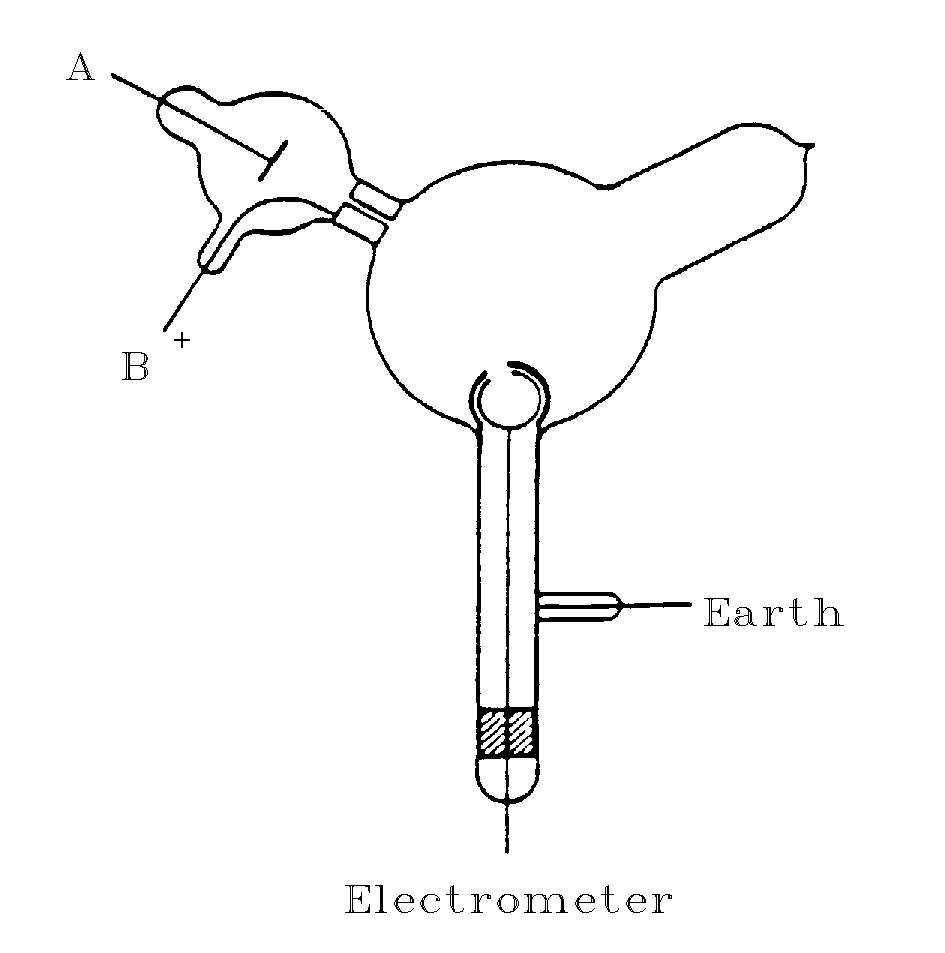
\includegraphics[width=3.17361in,height=3.2in]{images/02_thomson/image007.png}
  \end{center}
  \vspace*{-5mm}
  \caption{}
  \label{fig:thomson_1}
\end{figure}
  

Two coaxial cylinders (Fig.~\ref{fig:thomson_1}) with slits in them are placed in a bulb
connected with the discharge-tube; the cathode rays from the cathode A
pass into the bulb through a slit in a metal plug fitted into the neck
of the tube; this plug is connected with the anode and is put to earth.
The cathode rays thus do not fall upon the cylinders unless they are
deflected by a magnet. The outer cylinder is connected with the earth,
the inner with the electrometer. When the cathode rays (whose path was
traced by the phosphorescence on the glass) did not fall on the slit,
the electrical charge sent to the electrometer when the induction-coil
producing the rays was set in action was small and irregular; when,
however, the rays were bent by a magnet so as to fall on the slit there
was a large charge of negative electricity sent to the electrometer. I
was surprised at the magnitude of the charge; on some occasions enough
negative electricity went through the narrow slit into the inner
cylinder in one second to alter the potential of a capacity of 1.5
microfarads by 20 volts. If the rays were so much bent by the magnet
that they overshot the slits in the cylinder, the charge passing into
the cylinder fell again to a very small fraction of its value when the
aim was true. Thus this experiment shows that however we twist and
deflect the cathode rays by magnetic forces, the negative
electrification is indissolubly connected with the cathode rays.

When the rays are turned by the magnet so as to pass through the slit
into the inner cylinder, the deflexion of the electrometer connected
with this cylinder increases up to a certain value, and then remains
stationary although the rays continue to pour into the cylinder. This is
due to the fact that the gas in the bulb becomes a conductor of
electricity when the cathode rays pass through it, and thus, though the
inner cylinder is perfectly insulated when the rays are not passing, yet
as soon as the rays pass through the bulb the air between the inner
cylinder and the outer one becomes a conductor, and the electricity
escapes from the inner cylinder to the earth. Thus the charge within the
inner cylinder does not go on continually increasing; the cylinder
settles down into a state of equilibrium in which the rate at which it
gains negative electricity from the rays is equal to the rate at which
it loses it by conduction through the air. If the inner cylinder has
initially a positive charge it rapidly loses that charge and acquires a
negative one; while if the initial charge is a negative one, the
cylinder will leak if the initial negative potential is numerically
greater than the equilibrium value.

\subsection*{Deflexion of the Cathode Rays by an Electrostatic Field}

An objection very generally urged against the view that the cathode rays
are negatively electrified particles, is that hitherto no deflexion of
the rays has been observed under a small electrostatic force, and though
the rays are deflected when they pass near electrodes connected with
sources of large differences of potential, such as induction-coils or
electrical machines, the deflexion in this case is regarded by the
supporters of the ætherial theory as primarily due to the discharge
passing between the electrodes, and not primarily to the electrostatic
field. Hertz made the rays travel between two parallel plates of metal
placed inside the discharge-tube, but found that they were not deflected
when the plates were connected with a battery of storage-cells; on
repeating this experiment I at first got the same result, but subsequent
experiments showed that the absence of deflexion is due to the
conductivity conferred on the rarefied gas by the cathode rays. On
measuring this conductivity it was found that it diminished very rapidly
as the exhaustion increased; it seemed then that on trying Hertz's
experiment at very high exhaustions there might be a chance of detecting
the deflexion of the cathode rays by an electrostatic force.

The apparatus used is represented in Figure \ref{fig:thomson_2}.

\begin{figure}[h]
  \begin{center}
    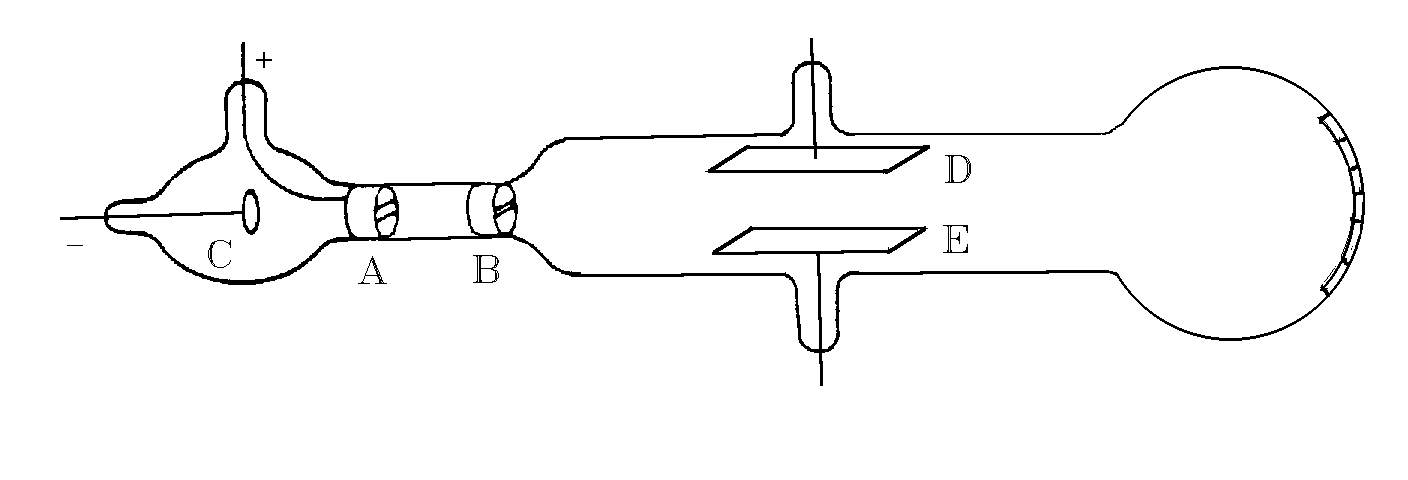
\includegraphics[width=4.69333in,height=1.6in]{images/02_thomson/image009.png}
  \end{center}
  \vspace*{-10mm}
  \caption{}
  \label{fig:thomson_2}
\end{figure}

The rays from the cathode C pass through a slit in the anode A, which is
a metal plug fitting tightly into the tube and connected with the earth;
after passing through a second slit in another earth-connected metal
plug B, they travel between two parallel aluminium plates about 5 cm
long by 2 broad and at a distance of 1.5 cm apart; they then fall on the
end of the tube and produce a narrow well-defined phosphorescent patch.
A scale pasted on the outside of the tube serves to measure the
deflexion of this patch. At high exhaustions the rays were deflected
when the two aluminium plates were connected with the terminals of a
battery of small storage-cells; the rays were depressed when the upper
plate was connected with the negative pole of the battery, the lower
with the positive, and raised when the upper plate was connected with
the positive, the lower with the negative pole. The deflexion was
proportional to the difference of potential between the plates, and I
could detect the deflexion when the potential-difference was as small as
two volts. It was only when the vacuum was a good one that the deflexion
took place, but that the absence of deflexion is due to the conductivity
of the medium is shown by what takes place when the vacuum has just
arrived at the stage at which the deflexion begins. At this stage there
is a deflexion of the rays when the plates are first connected with the
terminals of the battery, but if this connexion is maintained the patch
of phosphorescence gradually creeps back to its undeflected position.
This is just what would happen if the space between the plates were a
conductor, though a very bad one, for then the positive and negative
ions between the plates would slowly diffuse, until the positive plate
became coated with negative ions, the negative plate with positive ones;
thus the electric intensity between the plates would vanish and the
cathode rays be free from electrostatic force.\\
\centerline{* * *}
%
\subsection*{Magnetic Deflexion of the Cathode Rays in Different Gases}
%
\centerline{* * *}

As the cathode rays carry a charge of negative electricity, are
deflected by an electrostatic force as if they were negatively
electrified, and are acted on by a magnetic force in just the way in
which this force would act on a negatively electrified body moving along
the path of these rays, I can see no escape from the conclusion that
they are charges of negative electricity carried by particles of matter.
The next question arises, What are these particles? are they atoms, or
molecules, or matter in a still finer state of subdivision? To throw
some light on this point, I have made a series of measurements of the
ratio of the mass of these particles to the charge carried by it. To
determine this quantity, I have used two independent methods.\footnote{{[}We
  shall consider only the second and more accurate of Thomson's two
  methods.{]}}\\
\centerline{* * *}

I shall describe another method of measuring\footnote{{[}In the
  following, $m$ and $e$ are the mass and charge,
  respectively, and $v$ is the velocity, of a cathode ray particle.
  All of the electric quantities here are expressed in the
  \emph{electromag-netic system of units} (e.m.u.). Thus $e$ is in
  \emph{abcoulombs,} and so on. See Appendix (p.~\pageref{ch:appendix}).{]}} the
quantities $m/e$ and $v$ of an entirely different kind from
the preceding; this method is based upon the deflexion of the cathode
rays in an electrostatic field. If we measure the deflexion experienced
by the rays when traversing a given length under a uniform electric
intensity, and the deflexion of the rays when they traverse a given
distance under a uniform magnetic field, we can find the values of
$m/e$ and $v$ in the following way:---

Let the space passed over by the rays under a uniform electric intensity
\emph{F} be \emph{l},\footnote{{[}Thus \emph{l} is the length of the
  parallel plates D and E in Figure \ref{fig:thomson_2}.{]}} the time taken for the rays
to traverse this space is $l/v$, the {[}component of the final{]}
velocity in the direction of \emph{F} is therefore\footnote{{[}For this and the next expression 
see footnote \ref{fn:thomson_6}, which follows.{]}}
%
\begin{equation*}
\frac{Fe}{m} \cdot \frac{l}{v} 
\end{equation*}
%
so that $\theta$, the angle through which the rays are deflected when
they leave the electric field and enter a region free from electric
force, is given by the equation\footnote{\label{fn:thomson_6}{[}The force on the particle is always vertical and of
  magnitude $Fe$. When applied for a time $l/v$ it will impart
  a final vertical velocity $v'$, given by $l/v$ times the
  vertical acceleration, which is $Fe/m$; thus
\begin{equation*}
v' = \frac{Fe}{m} \frac{l}{v}.
\end{equation*}
  Then the vector resultant of horizontal velocity $v$ and vertical
  velocity $v'$ will be directed at an angle $\theta$ such that
\begin{equation*}
\tan{\theta} = \frac{v'}{v} = \frac{Fe}{m} \cdot \frac{l}{v^2}
\end{equation*}
  Moreover for small angles, $\tan{\theta}$ is nearly equal to
  $\theta$ (measured in radians); hence the formula in the text.{]}}
%
\begin{equation*}
\theta = \frac{Fe}{m} \cdot \frac{l}{v^2}.
\end{equation*}
%
If, instead of the electric intensity, the rays are acted on by a
magnetic force $H$ at right angles to the rays, and extending
across the distance $l$, then the {[}component of the final{]}
velocity at right angles to the original path of the rays is\footnote{{[}A charge $e$ (e.m.u.), moving with velocity $v$
  at right angles to the direction of a magnetic field $H$, will
  experience a force \emph{f}~=~\emph{Hev}, directed per\-pen\-dic\-u\-larly to
  both $v$ and $H$. (For a discussion see the Note at the end of this chapter, p.~\pageref{n:thomson}.) Now since \emph{a}~=~\emph{f}/\emph{m} and
  \emph{t}~=~\emph{l}/$v$, the charge will attain a (component of
  the) final velocity $v' = at = \frac{f}{m} \frac{l}{v}$ in the direction per\-pen\-dic\-u\-lar to $v$ and
  $H$. Substitution yields the expression cited.{]}}
%
\begin{equation*}
\frac{Hev}{m} \cdot \frac{l}{v},
\end{equation*}
%
so that $\phi$, the angle through which the rays are deflected when
they leave the magnetic field, is given by the equation\footnote{{[}Obtained by taking the ratio of vertical to horizontal
  components of velocity, just as was done previously for angle
  $\theta$.{]}}
%
\begin{equation*}
\phi = \frac{He}{m} \cdot \frac{l}{v}.
\end{equation*}
%
From these equations we get
\begin{equation*}
v = \frac{\phi}{\theta} \frac{F}{H} \quad \text{and} \quad \frac{m}{e} = \frac{H^{2}\theta l}{F\phi^2}.
\end{equation*}
In the actual experiments $H$ was adjusted so that $\phi =\theta$; in this case the equations become
\begin{equation*}
v = \frac{F}{H} \quad \text{and} \quad 
\frac{m}{e} = \frac{H^{2}l}{F\theta}.
\end{equation*}

The apparatus used to measure $v$ and $m/e$ by this means is
that represented in Figure \ref{fig:thomson_2}. The electric field was produced by
connecting the two aluminium plates to the terminals of a battery of
storage-cells. The phosphorescent patch at the end of the tube was
deflected, and the deflexion measured by a scale pasted to the end of
the tube. As it was necessary to darken the room to see the
phosphorescent patch, a needle coated with luminous paint was placed so
that by a screw it could be moved up and down the scale; this needle
could be seen when the room was darkened, and it was moved until it
coincided with the phosphorescent patch. Thus, when light was admitted,
the deflexion of the phosphorescent patch could be measured.

The magnetic field was produced by placing outside the tube two coils
whose diameter was equal to the length of the plates\ldots.\footnote{{[}We here 
  omit Thomson's description of his method of measuring the magnetic
  field.{]}}\\
\centerline{* * *}

A series of experiments was made to see if the electrostatic deflexion
was proportional to the electric intensity between the plates; this was
found to be the case. In the following experiments the current through
the coils was adjusted so that the electrostatic deflexion was the same
as the magnetic:---
\begin{table}[htp]\label{tbl:thomson_air}
\caption{}
\label{tbl:thomson_1}
\centering
%\begin{center}
\begin{tabular}{l*{6}{c}} % uses code from booktabs package to duplicate formatting in original paper
%\multicolumn{6}{c}{TABLE 1}\\[2pt] % This line no longer needed with the use of the caption command.
\toprule
\addlinespace[2pt]
\emph{Gas.} & $\theta.$ & $H.$ & $F.$ & $l.$ & $m/e.$ & $v.$\\
\cmidrule(lr){1-1}\cmidrule(lr){2-2}\cmidrule(lr){3-3}\cmidrule(lr){4-4}\cmidrule(lr){5-5}\cmidrule(lr){6-6}\cmidrule(lr){7-7}
\addlinespace[2pt]
Air           & 8/100   & 5.5 & $1.5\!\times\!{10^{10}}$ & 5 & $1.3\!\times\!{10^{-7}}$ & $2.8\!\times\!{10^9}$\\
Air           & 9.5/100 & 5.4 & $1.5\!\times\!{10^{10}}$ & 5 & $1.1\!\times\!{10^{-7}}$ & $2.8\!\times\!{10^9}$\\
Air           & 13/110  & 6.6 & $1.5\!\times\!{10^{10}}$ & 5 & $1.2\!\times\!{10^{-7}}$ & $2.3\!\times\!{10^9}$\\
Hydrogen      & 9/110   & 6.3 & $1.5\!\times\!{10^{10}}$ & 5 & $1.5\!\times\!{10^{-7}}$ & $2.5\!\times\!{10^9}$\\
Carbonic acid & 11/110  & 6.9 & $1.5\!\times\!{10^{10}}$ & 5 & $1.5\!\times\!{10^{-7}}$ & $2.2\!\times\!{10^9}$\\
Air           & 6/110   & 5   & $1.8\!\times\!{10^{10}}$ & 5 & $1.3\!\times\!{10^{-7}}$ & $3.6\!\times\!{10^9}$\\
Air           & 7/110   & 3.6 & $1\!\times\!{10^{10}}$   & 5 & $1.1\!\times\!{10^{-7}}$ & $2.8\!\times\!{10^9}$\\
\bottomrule
\end{tabular}
%\end{center}
\end{table}

The cathode in the first five experiments was aluminium, in the last two
experiments it was made of platinum; in the last experiment Sir William
Crookes's method of getting rid of the mercury vapour by inserting tubes
of pounded sulphur, sulphur iodide, and copper filings between the bulb
and the pump was adopted. In the calculation of $m/e$ and $v$
no allowance has been made for the magnetic force due to the coil in the
region outside the plates; in this region the magnetic force will be in
the opposite direction to that between the plates, and will tend to bend
the cathode rays in the opposite direction: thus the effective value of
H will be smaller than the value used in the equations, so that the
values of $m/e$ are larger and those of $v$ less than they
would be if this correction were applied\ldots.\footnote{{[}The value of
  \emph{m}/$e$ accepted today is $0.5685\!\times\!10^{-7}$ g/abC, less than
  half the average of the values given in Thomson's Table \ref{tbl:thomson_1} above. Thomson
  acknowledges that he has neglected the magnetic field \emph{outside}
  the parallel plates. Although he does not appear to regard that as a
  serious omission, it may in fact account for much of the discrepancy
  between his results and subsequent determinations.{]}}

From these determinations we see that the value of \emph{m/e} is
independent of the nature of the gas, and that its value $10^{-7}$ is very
small compared with the value $10^{-4}$, which is the smallest value of this
quantity previously known, and which is the value for the hydrogen ion
in electrolysis.\footnote{{[}Thomson here alludes to the results of
  electrolysis experiments such as our electroplating exercise: that one
  gram-equivalent weight of any element is associated with a charge of
  96,500 coulombs (9,650 abcoulombs). Then since 1 gram is the
  gram-equivalent weight of hydrogen, the quotient \emph{m/e} for
  hydrogen will be 1/9,650 g/abC, or approximately $10^{‑4}$, as Thomson
  cites.{]}}

Thus for the carriers of the electricity in the cathode rays $m/e$
is very small compared with its value in electrolysis. The smallness of
$m/e$ may be due to the smallness of $m$ or the largeness of
$e$, or to a combination of these two. That the carriers of the
charges in the cathode rays are small compared with ordinary molecules
is shown, I think, by Lenard's results as to the rate at which the
brightness of the phosphorescence produced by these rays diminishes with
the length of path traveled by the ray. If we regard this
phosphorescence as due to the impact of the charged particles, the
distance through which the rays must travel before the phosphorescence
fades to a given fraction (say, $1/e$, where $e = 2.71$)
of its original intensity, will be some moderate multiple of the mean
free path.\footnote{{[}Here, $e$ is the
  base of the natural log system, approximately 2.71, and should not be
  confused with $e$, the charge carried by a cathode ray
  ``corpuscle.'' The \emph{mean free path} of a molecule in a gas is the
  average distance it can travel before colliding with another molecule.
  For air at atmospheric pressure this distance is of the order of one
  millionth of 1 cm.{]}} Now Lenard found that this distance depends
solely upon the density of the medium, and not upon its chemical nature
or physical state. In air at atmospheric pressure the distance was about
half a centimetre, and this must be comparable with the mean free path
of the carriers through air at atmospheric pressure. But the mean free
path of the molecules of air is a quantity of quite a different order.
The carrier, then, must be small compared with ordinary molecules.\\
\centerline{* * *}

The explanation which seems to me to account in the most simple and
straight\-for\-ward manner for the facts is founded on a view of the
constitution of the chemical elements which has been favourably
entertained by many chemists: this view is that the atoms of the
different chemical elements are different aggregations of atoms of the
same kind. In the form in which this hypothesis was enunciated by
Prout,\footnote{{[}William Prout (1785-1850), English chemist and
  physician, pointed out in an anonymous article in the \emph{Annals of
  Philosophy} in 1815 that the atomic weights of a number of elements
  are multiples of that of hydrogen. In a second article in the
  following year he suggested that hydrogen was the ``prime matter'' of
  the ancients.{]}} the atoms of the different elements were hydrogen
atoms; in this precise form the hypothesis is not tenable, but if we
substitute for hydrogen some unknown primordial substance X, there is
nothing known which is inconsistent with this hypothesis\ldots.

If, in the very intense electric field in the neighborhood of the
cathode, the molecules of the gas are dissociated and are split up, not
into the ordinary chemical atoms, but into these primordial atoms, which
we shall for brevity call corpuscles; and if these corpuscles are
charged with electricity and projected from the cathode by the electric
field, they would behave exactly like the cathode rays. They would
evidently give a value of \emph{m/e} which is independent of the nature
of the gas and its pressure, for the carriers are the same whatever the
gas may be\ldots.

Thus we have in the cathode rays matter in a new state, a state in which
the sub\-di\-vi\-sion of matter is carried very much further than in the
ordinary gaseous state: a state in which all matter---that is, matter
derived from different sources such as hydrogen, oxygen, \&c.---is of
one and the same kind; this matter being the substance from which all
the chemical elements are built up.\\
\centerline{* * *}
%
\section*{Experiment: The Ratio of Charge to Mass in Cathode Rays}

The cathode-ray tube de\-scribed here operates on the same principles as
does that de\-scribed by Thomson. However, the experiment is made somewhat
more elegant by causing the cathode-ray particles to orbit in a circular
path under the action of the magnetic field alone. This happens because
in a magnetic field $H$ the force on a charge $e$ moving with
velocity $v$ is always per\-pen\-dic\-u\-lar to both $H$ and $v$.
Thus if $v$ is initially per\-pen\-dic\-u\-lar to $H$ and if $H$
is uniform, the forces on $e$ will always deflect it in a single
plane per\-pen\-dic\-u\-lar to $H$, as diagrammed in Figure
\ref{fig:thomson_3}.\footnote{If in the figure the indicated direction for the force
  \emph{f} seems to be reversed, recall that the charge on the
  hypothetical cathode-ray particle is \emph{negative}.} Moreover, since
force $f$ is also normal to $v$, the charge $e$ will
never be accelerated in the direction of its motion, and $v$ will
therefore remain constant in magnitude and vary only in direction. But
these are exactly the conditions for circular motion with constant
speed; in such an orbit the force is always normal to the velocity and
is directed to a virtual center, O.

\begin{figure}[htp]
\centering
  %\begin{center}
    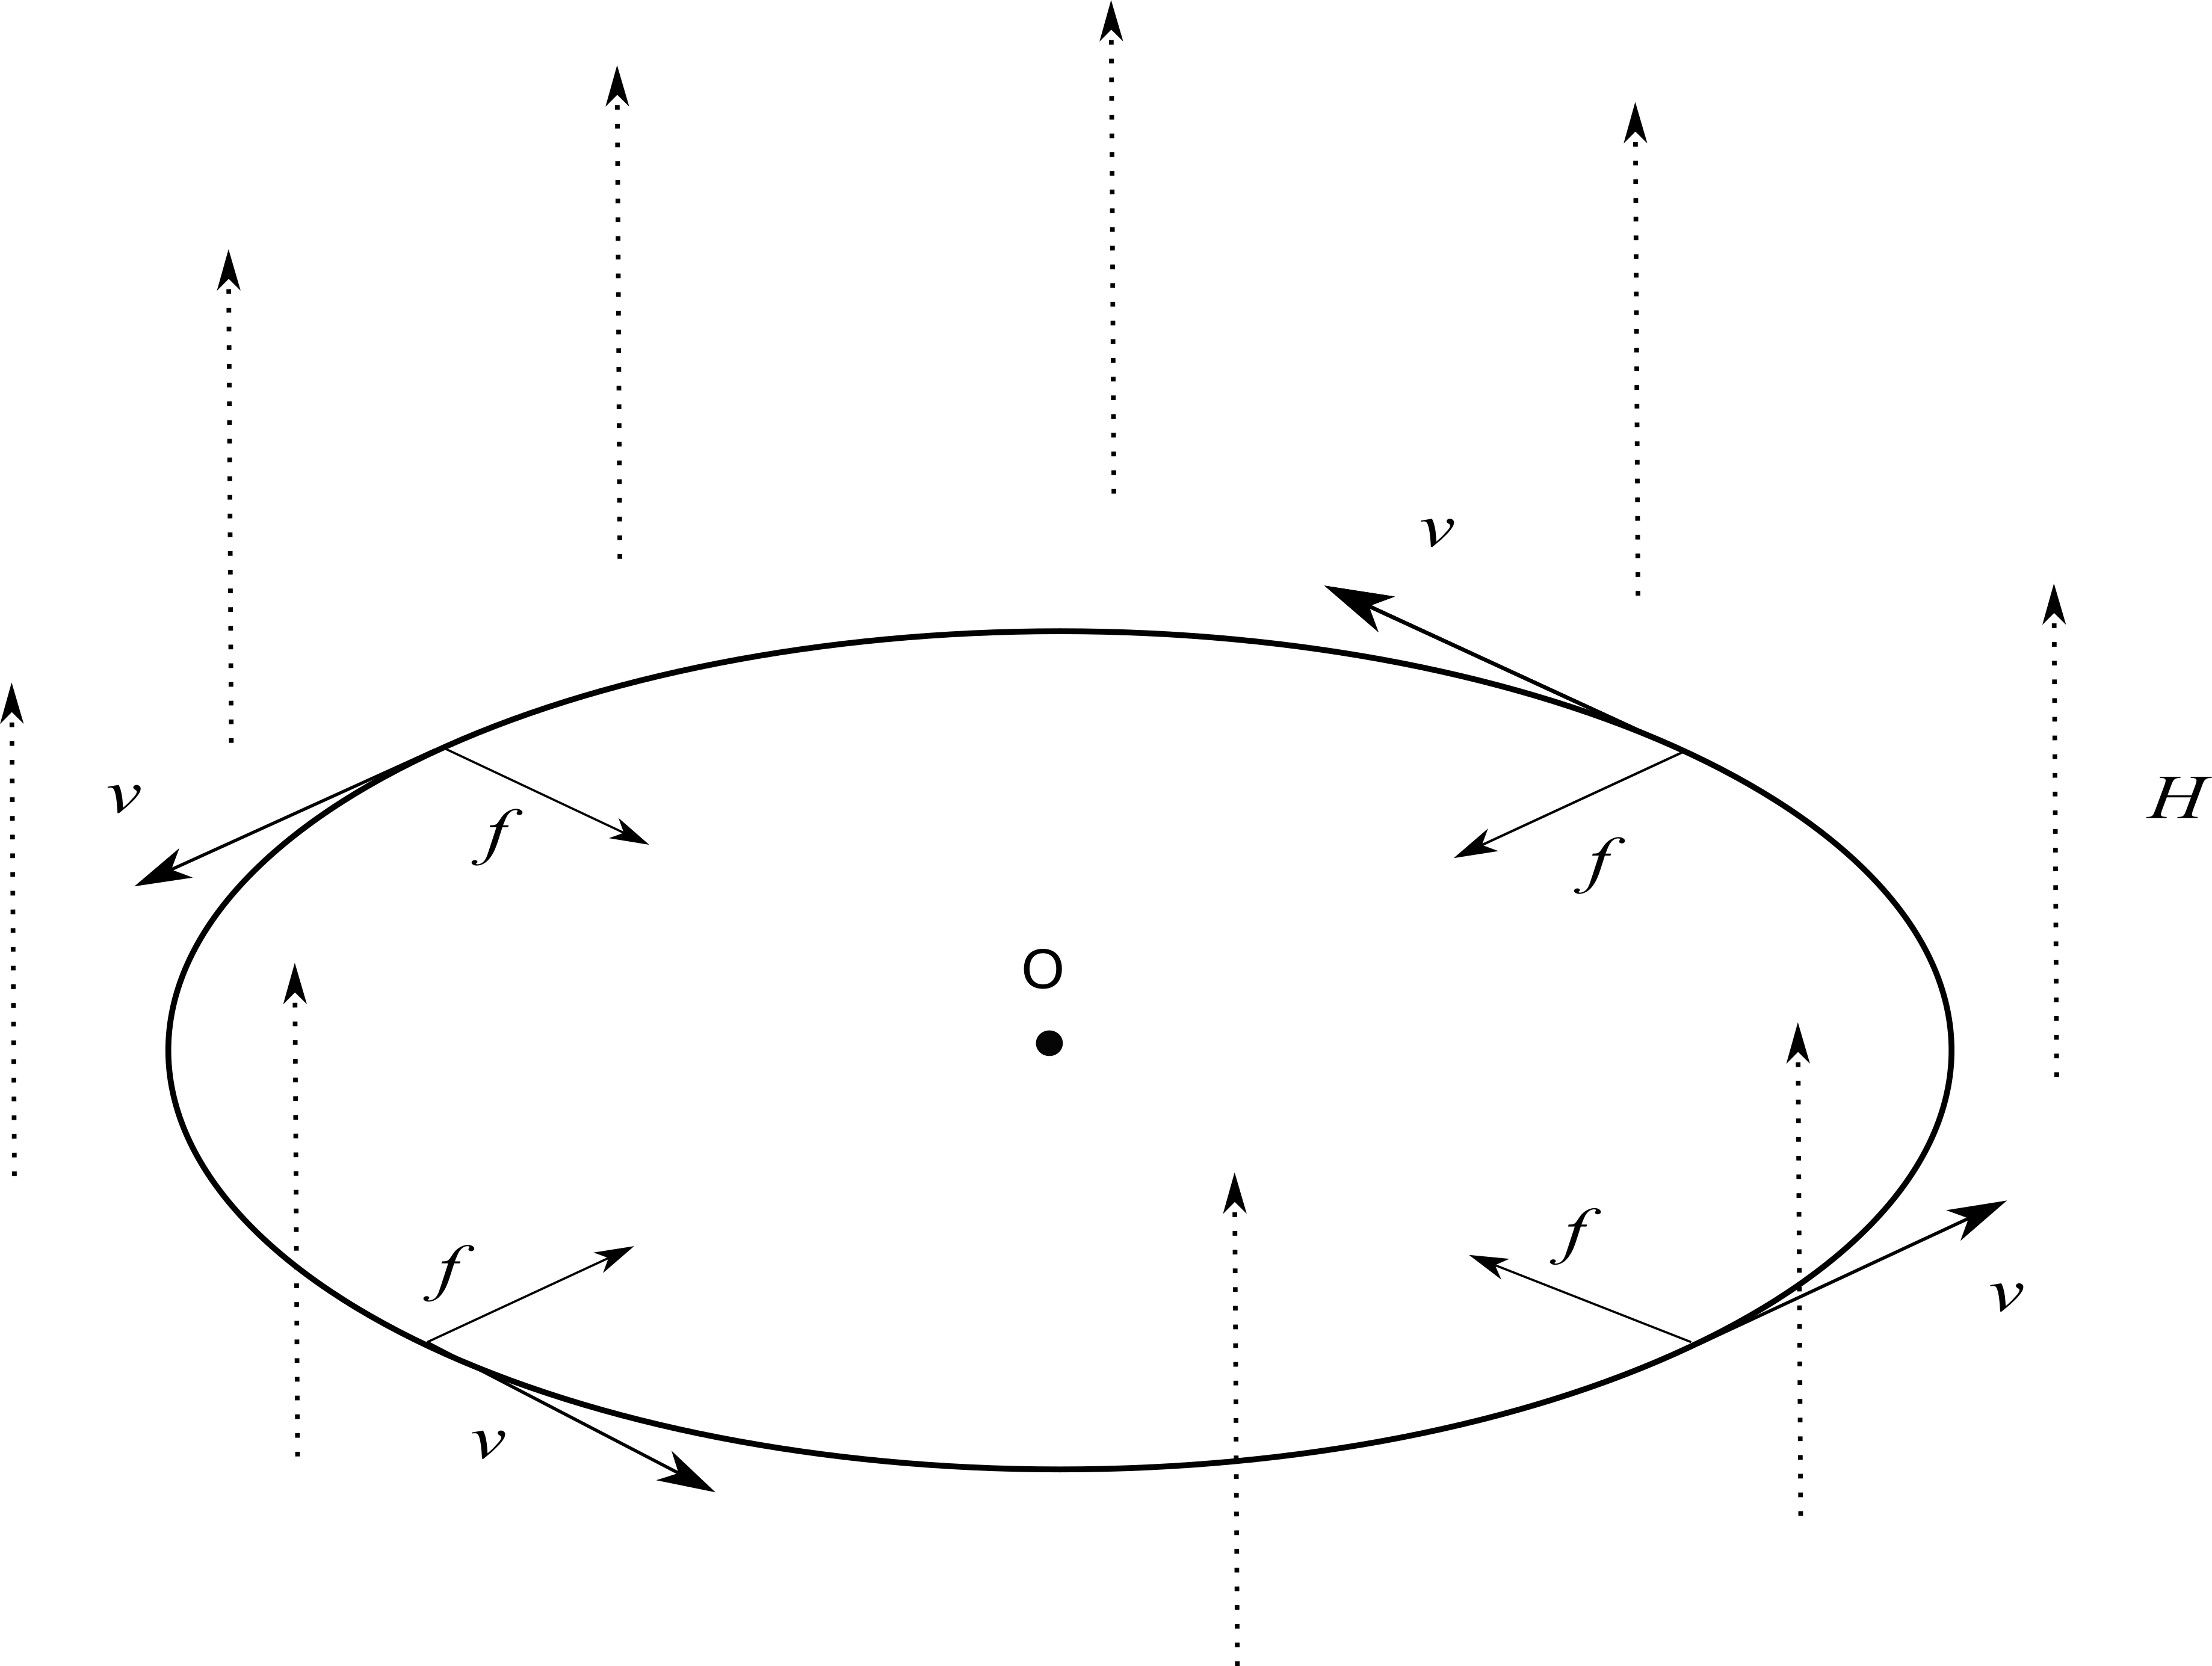
\includegraphics[width=0.75\textwidth]{images/02_thomson/image099.png}
  %\end{center}
\caption{}
\label{fig:thomson_3}
\end{figure}

Now the acceleration $a$ towards the center of circular motion is
$a = v^2/r$,\footnote{Cf. Newton, \emph{Principia},
  Prop.\ IV, Corollary 1.} so that the central force will be given by
%
\begin{equation}
f = ma = mv^2/r.\label{eq:thomson_1}
\end{equation}
%
In the present case the force $f$ is supplied by the magnetic field
and is therefore\footnote{See Note at the end of this chapter (p.~\pageref{n:thomson}).}
\begin{equation}
f = Hev\label{eq:thomson_2}
\end{equation}
(compare Thomson's equation for magnetic deflection). Combining
equations \eqref{eq:thomson_1} and \eqref{eq:thomson_2}, we find
\begin{equation}
\frac{e}{m} = \frac{v}{rH};\label{eq:thomson_3}
\end{equation}
the ratio $e/m$ will thus be known if $r$, $H$, and
$v$ are known. We use a tube in which several radii $r$
are marked on a phosphor-coated scale running the length of the tube; 
the magnetic field $H$ is adjusted
until the ray orbit intersects the scale at a predetermined marking indicating 
the diameter (e.g., 10 cm), and thus $r$ is
known. It remains only to determine $H$ and $v$.

\begin{figure}[htp]
    \centering
    \begin{minipage}{0.5\textwidth}
        \centering
        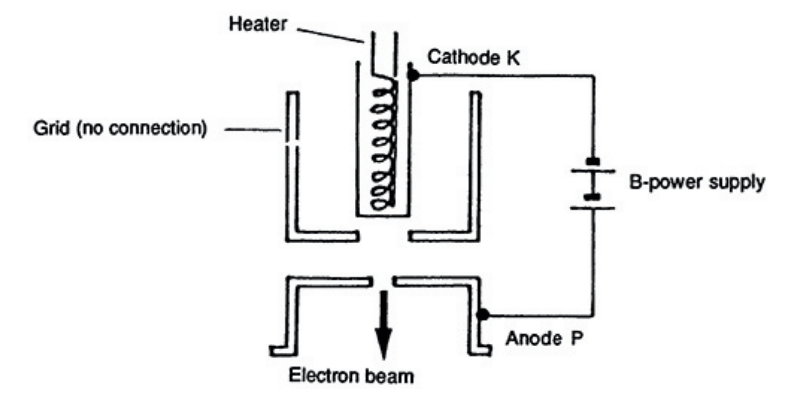
\includegraphics[width=\textwidth]{images/02_thomson/gun.png} % first figure itself
        %\caption{}
    \end{minipage}\hfill
    \begin{minipage}{0.5\textwidth}
        \centering
        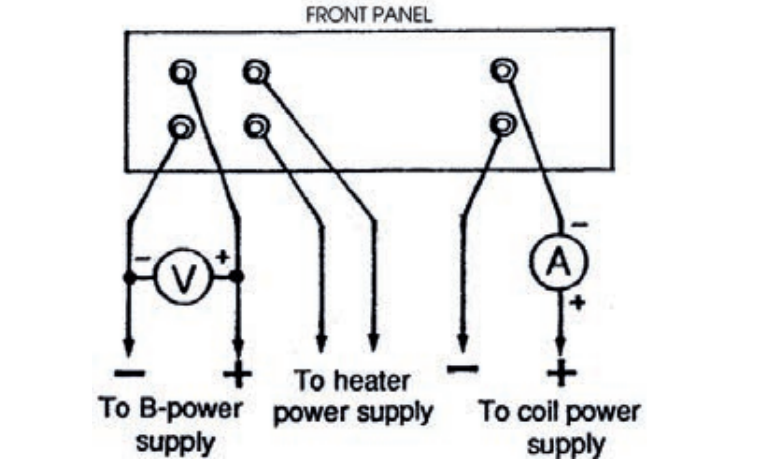
\includegraphics[width=\textwidth]{images/02_thomson/power-supply.png} % second figure itself
        %\caption{}
    \end{minipage}
    \caption{}
    \label{fig:thomson_4}
\end{figure}

%\begin{figure}[htp]
%\centering
%  %\begin{center}
%    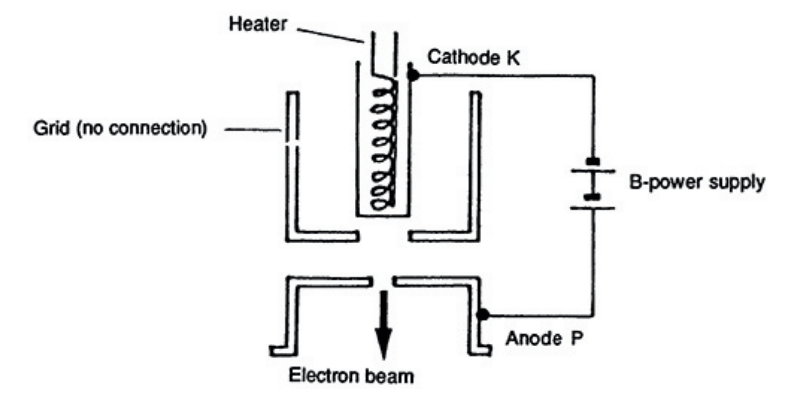
\includegraphics[width=2.63in,height=1.36667in]{images/02_thomson/gun.png}
%  %\end{center}
%\end{figure}

The tube with its connections is diagrammed in Figure \ref{fig:thomson_4}. It contains
an anode and a heated cathode. A power supply maintains the anode at a positive
potential with respect to the cathode, so that negative particles emitted
by it are accelerated towards the anode and pass through the slit with
considerable velocity. Current is run through a pair of coils that surrounds the tube, arranged so that 
their magnetic fields combine to form a nearly uniform field in the region of the tube. The beam of 
particles is indicated by the glow of vapor in the tube; coil current is adjusted until 
the orbit of the particles lines up with one of the marks for measurement.

%\begin{figure}[h]
%  \begin{center}
%    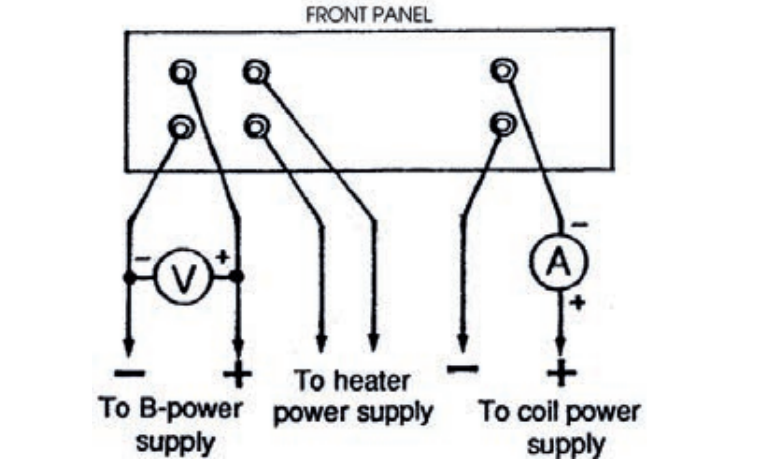
\includegraphics[width=2.59in,height=1.53667in]{images/02_thomson/power-supply.png}
%  \end{center}
%\end{figure}

Energy considerations determine the velocity $v$. Since particles
emitted from the cathode are accelerated to the anode, they gain kinetic
energy equal to the work done by the electric field on them. This work
equals the product of the potential difference and the charge on the
particle,\footnote{See Appendix (p.~\pageref{ch:appendix}).} so that in electromagnetic
units ($V$ in abvolts and $e$ in abcoulombs), we have
%
\begin{equation}
Ve = \frac{1}{2}mv^2 \quad\text{or}\quad v = \sqrt{\frac{2Ve}{m}}.\label{eq:thomson_4}
\end{equation}
%
If $V$ represents the measurement in \emph{volts} as per our
meters, a conversion factor must be introduced ($1$ volt = $10^8$ abvolts),
and the equation becomes
\begin{equation}
v = \sqrt{\frac{2V_{volt}e\cdot{10^8}}{m}}\label{eq:thomson_5}
\end{equation}
Substitution of this value in equation (3) yields for $e/m$:
\begin{equation}
\frac{e}{m} = \frac{2V_{volt}}{r^2H^2}\cdot 10^8 \:\text{abC/g.}\label{eq:thomson_6}
\end{equation}

\begin{wrapfigure}[11]{R}{2.75in}
\centering
  %\begin{center}
    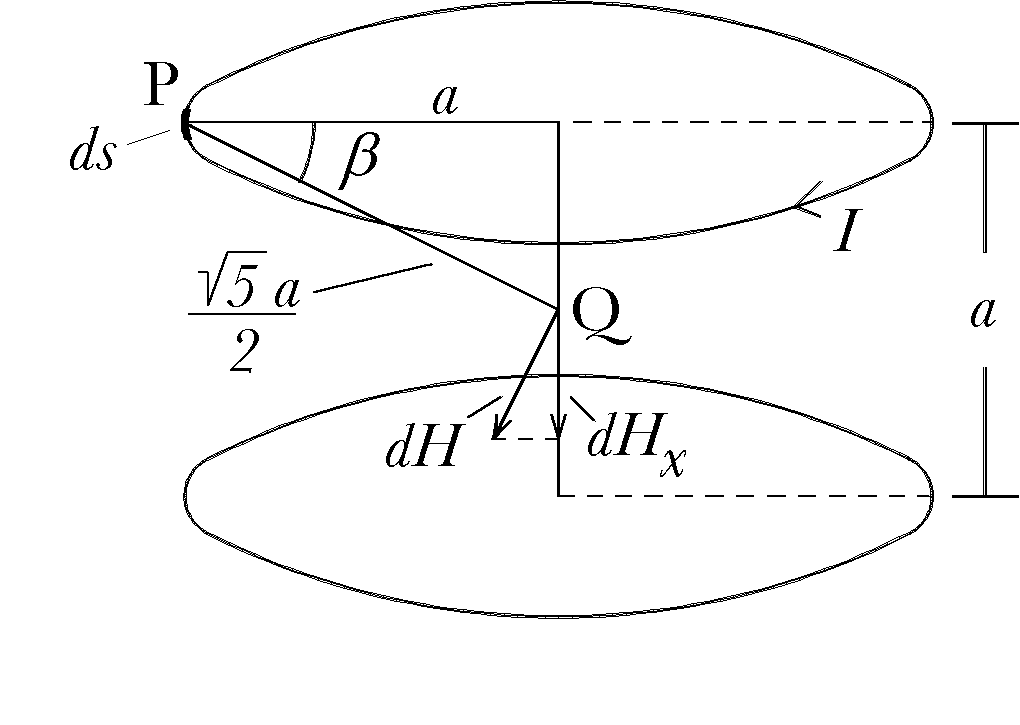
\includegraphics[width=2.72153in,height=1.93056in]{images/02_thomson/image039.png}
  %\end{center}
\end{wrapfigure}

%\includegraphics[width=2.72153in,height=1.93056in]{media/image23.png}

Finally, the magnetic field $H$ must be found. The pair of coils we
use, known as Helmholtz coils, is so designed that the distance between
them is equal to the coil radius $a$. (This makes the magnetic field
between the coils relatively uniform.) The tube is placed at Q,
which is at a distance $a/2$ from the center of each coil. The
contribution $dH$ that a current element $I\,ds$ at P makes to
the field at Q will be
\begin{equation*}
dH = \frac{I\,ds}{PQ^2} = \frac{I\,ds}{(5/4)a^2} = \frac{4}{5}\frac{I\,ds}{a^2}
\end{equation*}
(using the Pythagorean Theorem to give us PQ$^2$). As
successive current elements are considered, components of \emph{dH}
per\-pen\-dic\-u\-lar to the axis cancel one another, so that only axial
components $dH_x$ are effective. But
\begin{equation*}
\cos{\beta} = a/PQ = 2/\sqrt{5},
\end{equation*}
whence
\begin{equation}
dH_x = dH \cos{\beta} = \frac{2}{\sqrt{5}}dH = \frac{8}{5\sqrt{5}}\frac{I\,ds}{a^2}.\label{eq:thomson_7}
\end{equation}
Integrating, we obtain
\begin{equation*}
H = \int_{0}^{2\pi{a}} \frac{8}{5\sqrt{5}}\frac{I}{a^2}\,ds = \frac{8}{5\sqrt{5}}\frac{2\pi aI}{a^2} = \frac{16\pi I}{5\sqrt{5}a}.
\end{equation*}
For \emph{two} coils of \emph{N} turns each, therefore,
\begin{equation*}
H = \frac{32\pi IN}{5\sqrt{5}a}.
\end{equation*}
If the current $I$ is stated in \emph{amperes} as per our meter
readings, the above equation becomes
\begin{equation}
H = \frac{3.2\pi NI_{amp}}{5\sqrt{5}a}.\label{eq:thomson_8}
\end{equation}
For our coils, $N$ = 130.

Thus we use equation \eqref{eq:thomson_8} to determine the magnetic field $H$; then
we substitute this value into equation \eqref{eq:thomson_6} to determine the
charge-to-mass ratio $e/m$.

\subsubsection*{Operation}

When the apparatus is wired, orient the coils so their axis is aligned
with magnetic north in the room (use a compass for
this purpose). Slowly raise $V$, the anode voltage, to some value between 200 and 300 volts. 
Record this voltage, and vary the coil current $I$ until the beam falls on one
of the markers. Half of this diameter will be your radius $r$ for equation \eqref{eq:thomson_6}. 
With known $I$ we calculate $H$ using equation
\eqref{eq:thomson_8}; then with known $H$ and $V$ and $r$ we calculate
$e/m$ using equation \eqref{eq:thomson_6}. It makes sense to determine $e/m$
several times using different radii and different voltages. Although by
our theory the values thus obtained ought to agree, in practice they may
differ. If so, look for any suggestive regularities in the differences;
for example, are measurements taken at higher voltages uniformly greater
or less than those taken at lower voltages? What might cause such an
effect?


\section*{Note: On Magnetic Fields and Moving Charged Bodies}\label{n:thomson}

A current-carrying wire, because of the magnetic field which it generates,
will exert a force on any magnet placed near it. By Newton's Third Law,
the magnet will necessarily exert \emph{an equal and opposite force back
on the wire}. Thus, magnetic fields exert force on current-carrying
wires. If a long straight wire carrying a current of 1 abampere is
placed in a perfectly uniform magnetic field of unit strength with the
field lines perpendicular to the wire, then it will experience \emph{a
force of one dyne for every centimeter of its length}. The force will be
perpendicular to both the wire and the field lines.

An analogous situation holds for \emph{moving charged bodies} in a
magnetic field. A body carrying 1 abcoulomb and moving at 1 centimeter
per second through a magnetic field of unit strength will experience a
force of \emph{1 dyne} perpendicular to both the field lines and the
direction of motion. We cannot argue rigorously for this here, but note
that in one second this charged body makes one abcoulomb ``flow'' a
distance of one centimeter---just as does a 1-cm-long wire carrying 1
abamp, which also would experience a force of one dyne. At any rate, in
general
\begin{equation*}
f = Hev ,
\end{equation*}
where $f$ is the force, $H$ is the magnetic field strength,
$e$ is the charge \emph{in abamperes} and $v$ is the velocity
in cm./sec.

For both the current-carrying wire and the moving charged particle, the
direction of the force is more or less conveniently given by the ``left
hand rule,'' also known as the ``\emph{fBI''} rule. Arrange the thumb,
forefinger and middle fingers on your left (your \emph{left}) hand so
that they are mutually perpendicular, like 3-dimensional coordinate
axes. Then your thumb will give the direction of \emph{f} the force if
your forefinger points in the direction of \emph{B} the magnetic field
and your middle finger in the direction of \emph{I} the current.
(Remember that for a cathode-ray current, \emph{I} is in the opposite
direction of the motion of the electrons, since they are negatively
charged.)
